\documentclass[10pt,a4paper]{article}

% -----------------------------------------------------------------------------
% MATHS MANTHAN | Class 10 Coordinate Geometry Handbook | 2026--27
% Self-contained publication-quality master formula & concept handbook.
% Strictly compliant with the rationalized CBSE Class 10 curriculum.
% Exactly 14 Pages with zero overfull boxes or unintended page overflow.
% -----------------------------------------------------------------------------

\usepackage[a4paper,top=12mm,bottom=15mm,left=15mm,right=15mm,footskip=8mm]{geometry}
\usepackage[T1]{fontenc}
\usepackage{lmodern}
\usepackage{microtype}
\usepackage{amsmath,amssymb}
\usepackage[table]{xcolor}
\usepackage{array,tabularx,booktabs}
\usepackage{graphicx}
\usepackage{eso-pic}
\usepackage{tikz}
\usetikzlibrary{calc,positioning,arrows.meta,shapes.geometric,patterns}
\usepackage[most]{tcolorbox}
\usepackage{enumitem}
\usepackage{fancyhdr}
\usepackage{lastpage}
\usepackage[hidelinks]{hyperref}
\usepackage{url}

% Compatibility fix for modern LaTeX/MiKTeX: colortbl + tabularx p-column alignment
\makeatletter
\let\insert@pcolumn\insert@column
\makeatother

% ============================================================================
% BRAND COLOR PALETTE — MATCHED TO THE MATHS MANTHAN STANDARD
% Primary navy: #001F49 | Brand gold: #D19029
% ============================================================================
\definecolor{primary}{RGB}{0,31,73}
\definecolor{brandnavy}{RGB}{0,31,73}
\definecolor{accent}{RGB}{209,144,41}
\definecolor{brandgold}{RGB}{209,144,41}
\definecolor{secondary}{RGB}{75,85,99}
\definecolor{lightgray}{RGB}{246,248,250}
\definecolor{accentlight}{RGB}{254,250,242}
\definecolor{primarylight}{RGB}{240,244,250}

\colorlet{navy}{primary}
\colorlet{blue}{primary!82!black}
\colorlet{gold}{accent}
\colorlet{goldpale}{accentlight}
\colorlet{bluepale}{primarylight}
\colorlet{ink}{secondary}
\colorlet{muted}{secondary}
\colorlet{linegray}{primary!25}
\colorlet{reddeep}{primary}
\colorlet{redpale}{lightgray}
\colorlet{green}{primary}
\colorlet{greenpale}{primarylight}

% Automatic low-opacity logo watermark on every page
\IfFileExists{mathsmanthan logo.png}{%
  \AddToShipoutPictureBG{%
    \begin{tikzpicture}[remember picture,overlay]
      \node[opacity=0.065] at (current page.center) {%
        \includegraphics[width=0.55\paperwidth,keepaspectratio]{mathsmanthan logo.png}%
      };
    \end{tikzpicture}%
  }%
}{}

\hypersetup{
  pdftitle={Class 10 Coordinate Geometry | Maths Manthan Handbook},
  pdfauthor={Maths Manthan Tuition Classes},
  pdfsubject={CBSE Class 10 Mathematics, Academic Year 2026--27},
  pdfkeywords={Coordinate Geometry, Distance Formula, Section Formula, Midpoint, Collinearity, CBSE Class 10, Maths Manthan}
}

\setlength{\parindent}{0pt}
\setlength{\parskip}{2pt}
\renewcommand{\arraystretch}{1.15}
\setlist[itemize]{leftmargin=4.5mm,itemsep=1pt,topsep=1pt,parsep=0pt}
\setlist[enumerate]{leftmargin=5.5mm,itemsep=1pt,topsep=1pt,parsep=0pt}
\setlength{\tabcolsep}{4.5pt}
\emergencystretch=2em
\hfuzz=1pt

% ============================================================================
% HEADER / FOOTER
% ============================================================================
\newcommand{\TuitionName}{{\color{primary}MATHS} {\color{accent}MANTHAN}}
\newcommand{\TuitionSub}{{\color{primary}\textbullet\ \ \text{TUITION CLASSES}\ \ \textbullet}}
\newcommand{\ContactInfo}{e-mail: contact@mathsmanthan.co.in \quad$\vert$\quad Helpline: +91-8171546558}
\newcommand{\HandbookFooterTitle}{Class 10 Coordinate Geometry Handbook}

\pagestyle{fancy}
\fancyhf{}
\renewcommand{\headrulewidth}{0pt}
\renewcommand{\footrulewidth}{0.6pt}
\renewcommand{\footrule}{\hbox to\headwidth{\color{primary!30}\leaders\hrule height 0.6pt\hfill}}
\fancyfoot[L]{\footnotesize\href{https://mathsmanthan.co.in}{\textcolor{secondary}{\TuitionName\ $\vert$\ \HandbookFooterTitle}}}
\fancyfoot[R]{\footnotesize\textbf{\color{primary}Page \thepage\ of \pageref{LastPage}}\quad\textcolor{accent}{\textbf{Academic Year 2026--27}}}

\fancypagestyle{plain}{%
  \fancyhf{}
  \fancyfoot[L]{\footnotesize\href{https://mathsmanthan.co.in}{\textcolor{secondary}{\TuitionName\ $\vert$\ \HandbookFooterTitle}}}
  \fancyfoot[R]{\footnotesize\textbf{\color{primary}Page \thepage\ of \pageref{LastPage}}\quad\textcolor{accent}{\textbf{Academic Year 2026--27}}}
  \renewcommand{\headrulewidth}{0pt}
  \renewcommand{\footrulewidth}{0.6pt}
  \renewcommand{\footrule}{\hbox to\headwidth{\color{primary!30}\leaders\hrule height 0.6pt\hfill}}
}

% Reusable design components
\newcommand{\BrandMark}{%
  \IfFileExists{mathsmanthan logo.png}{%
    \includegraphics[width=22mm,height=22mm,keepaspectratio]{mathsmanthan logo.png}%
  }{%
    
\begin{tikzpicture}[baseline=-0.6ex]
      \fill[navy,rounded corners=2.2pt] (0,0) rectangle (1.45,1.05);
      \draw[gold,line width=1.2pt] (0.15,0.15)--(1.30,0.15);
      \node[text=white,font=\sffamily\bfseries\Large] at (0.725,0.59) {MM};
    \end{tikzpicture}%
  }%
}

\newcommand{\chapterbanner}[4]{%
  \begin{tcolorbox}[enhanced,colback=bluepale,colframe=bluepale,boxrule=0pt,arc=2mm,
    left=3.5mm,right=3.5mm,top=1.8mm,bottom=1.8mm]
    {\footnotesize\bfseries\color{gold}CHAPTER #1\hfill\color{blue}#4}\par\vspace{0.4mm}
    {\Large\bfseries\color{navy}#2}\par
    {\small\color{muted}#3}
  \end{tcolorbox}\vspace{0.8mm}
}

\newcommand{\subhead}[1]{%
  \vspace{1mm}{\large\bfseries\color{navy}#1}\par\vspace{0.3mm}
  {\color{gold}\rule{14mm}{1.2pt}}\par\vspace{0.8mm}
}

\newtcolorbox{formulaBox}[1][]{enhanced,breakable,colback=goldpale,colframe=gold!65!black,
  boxrule=0.5pt,arc=1.5mm,left=2.8mm,right=2.8mm,top=1.8mm,bottom=1.8mm,
  before skip=2pt,after skip=3pt,#1}
\newtcolorbox{conceptBox}[1][]{enhanced,breakable,colback=bluepale,colframe=blue!25,
  boxrule=0.4pt,arc=1.5mm,left=2.8mm,right=2.8mm,top=1.8mm,bottom=1.8mm,
  before skip=2pt,after skip=3pt,#1}
\newtcolorbox{warningBox}[1][]{enhanced,breakable,colback=redpale,colframe=reddeep!45,
  boxrule=0.45pt,arc=1.5mm,left=2.8mm,right=2.8mm,top=1.8mm,bottom=1.8mm,
  before skip=2pt,after skip=3pt,#1}
\newtcolorbox{successBox}[1][]{enhanced,breakable,colback=greenpale,colframe=green!35,
  boxrule=0.45pt,arc=1.5mm,left=2.8mm,right=2.8mm,top=1.8mm,bottom=1.8mm,
  before skip=2pt,after skip=3pt,#1}

\newcommand{\CoreTag}{\tcbox[colback=greenpale,colframe=green!40,boxrule=.3pt,arc=1mm,left=1.5mm,right=1.5mm,top=.5mm,bottom=.5mm]{\scriptsize\bfseries\color{green}CORE SYLLABUS}}
\newcommand{\ExamTag}{\tcbox[colback=bluepale,colframe=blue!25,boxrule=.3pt,arc=1mm,left=1.5mm,right=1.5mm,top=.5mm,bottom=.5mm]{\scriptsize\bfseries\color{blue}EXAM STRATEGY}}
\newcommand{\TrapTag}{\tcbox[colback=redpale,colframe=reddeep!40,boxrule=.3pt,arc=1mm,left=1.5mm,right=1.5mm,top=.5mm,bottom=.5mm]{\scriptsize\bfseries\color{reddeep}TRAP ALERT}}
\newcommand{\ReferenceTag}{\tcbox[colback=bluepale,colframe=blue!25,boxrule=.3pt,arc=1mm,left=1.5mm,right=1.5mm,top=.5mm,bottom=.5mm]{\scriptsize\bfseries\color{blue}QUICK REFERENCE}}

\begin{document}

% =============================================================================
% PAGE 1: STANDALONE INSTITUTIONAL COVER PAGE
% =============================================================================
\thispagestyle{fancy}
\vspace*{0mm}
\noindent
\makebox[0pt][l]{%
  \raisebox{-0.80cm}[0pt][0pt]{%
    \href{https://mathsmanthan.co.in}{\BrandMark}%
  }%
}%
\parbox{\textwidth}{%
  \centering
  \href{https://mathsmanthan.co.in}{%
    {\fontsize{23pt}{23pt}\selectfont\bfseries \TuitionName}\\[3pt]
    {\footnotesize\bfseries \TuitionSub}%
  }\\[2pt]
  {\scriptsize\color{secondary} \ContactInfo}
}

\vspace{4pt}
\noindent{\color{primary}\rule{0.72\textwidth}{1.5pt}}\hfill{\color{accent}\rule{0.26\textwidth}{1.5pt}}

\vspace{3mm}
\begin{center}
  {\large\bfseries\color{muted}CBSE CLASS 10 \;$\vert$\; MATHEMATICS}\\[3mm]
  {\fontsize{26}{30}\selectfont\bfseries\color{navy}COORDINATE GEOMETRY}\\[2mm]
  {\Large\color{blue}Master Concept, Formula \& Visual Problem-Solving Handbook}\\[2mm]
  {\large\color{gold}\bfseries Academic Year 2026--27}
\end{center}

\vspace{2.5mm}
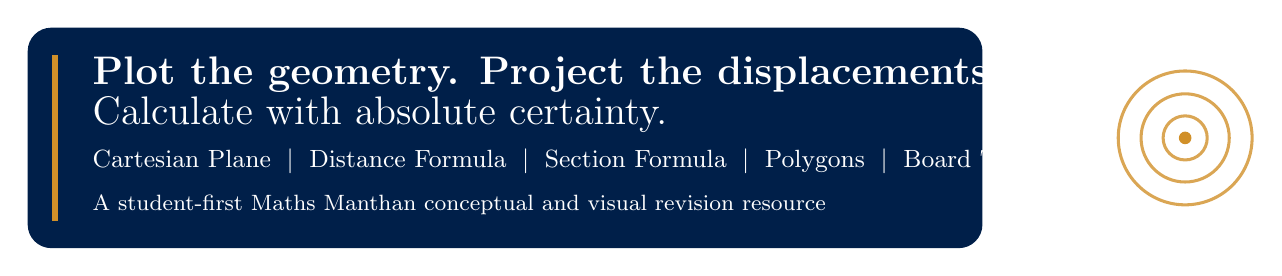
\begin{tikzpicture}
  \fill[navy,rounded corners=3mm] (0,0) rectangle (\textwidth,2.8);
  \draw[gold,line width=2pt] (0.35,0.35)--(0.35,2.45);
  \node[anchor=west,text=white,font=\bfseries\Large] at (0.7,2.2) {Plot the geometry. Project the displacements.};
  \node[anchor=west,text=white,font=\Large] at (0.7,1.7) {Calculate with absolute certainty.};
  \node[anchor=west,text=white,font=\small] at (0.7,1.1) {Cartesian Plane \;$\vert$\; Distance Formula \;$\vert$\; Section Formula \;$\vert$\; Polygons \;$\vert$\; Board Traps};
  \node[anchor=west,text=white!75,font=\footnotesize] at (0.7,0.55) {A student-first Maths Manthan conceptual and visual revision resource};
  \foreach \x/\r in {14.7/0.85,14.7/0.56,14.7/0.28} {\draw[gold!80,line width=1.1pt] (\x,1.4) circle (\r);}
  \fill[gold] (14.7,1.4) circle (0.08);
\end{tikzpicture}

\vspace{3mm}
\begin{minipage}[t]{0.48\textwidth}
  \begin{conceptBox}[title=What This Handbook Includes,fonttitle=\bfseries\color{navy}]
    \begin{itemize}
      \item Cartesian coordinate plane anatomy and projections
      \item Pythagorean derivation of the Distance Formula
      \item Geometric classification of triangles and quadrilaterals
      \item Rigorous similar-triangles derivation of Section Formula
      \item The $k:1$ parameterization and axis-intersection models
      \item Trisection mechanics, parallelogram diagonals, and centroid
    \end{itemize}
  \end{conceptBox}
\end{minipage}\hfill
\begin{minipage}[t]{0.48\textwidth}
  \begin{formulaBox}[title=Pedagogical Strategy: Foundations First,fonttitle=\bfseries\color{navy}]
    \raggedright Coordinate geometry bridges algebra and Euclidean geometry. Every coordinate $(x,y)$ represents signed perpendicular displacements from perpendicular reference axes. Never blindly memorize:
    $$\mathbf{\text{Distance} = \text{Hypotenuse of Right } \triangle}$$
    $$\mathbf{\text{Section Point} = \text{Weighted Center}}$$
    Always draw a rough sketch with signs before setting up equations!
  \end{formulaBox}
\end{minipage}

\vspace{1.5mm}
\begin{warningBox}[title=CBSE 2026--27 Curriculum Verification \& Rationalized Scope,fonttitle=\bfseries\color{navy}]
  \textbf{Official Scope (Prescribed \& Tested):} Concepts of coordinate geometry, graphs of linear equations, distance formula, section formula (internal division only), midpoint, and coordinates of points dividing a line segment in a given ratio. Geometrical applications to triangles and quadrilaterals.\\
  \textbf{Excluded / Deleted Topics (Non-Examinable):}
  \begin{itemize}
    \item \textbf{Area of a Triangle:} $\frac{1}{2}|x_1(y_2-y_3) + x_2(y_3-y_1) + x_3(y_1-y_2)|$ is \textbf{deleted from the syllabus}.
    \item \textbf{Collinearity via Area = 0:} Must NOT be used. Collinearity must be proved using the \textbf{Distance Sum Property} ($AB + BC = AC$) or the \textbf{Consistent Section Ratio Method}.
    \item \textbf{External Division:} Only internal division ($m_1, m_2 > 0$) is examinable.
  \end{itemize}
\end{warningBox}

\vfill
\begin{center}
  {\small\bfseries\color{navy}Maths Manthan Tuition Classes}\\
  {\footnotesize\color{muted}contact@mathsmanthan.co.in \quad$\vert$\quad +91-8171546558}\\
  {\footnotesize\url{https://mathsmanthan.co.in}}\\[1.5mm]
  {\scriptsize\color{muted}Prepared for learning and conceptual mastery \;--\; Strictly aligned with CBSE Class 10 Syllabus 2026--27.}
\end{center}

\newpage

% =============================================================================
% PAGE 2: MODULE 1 — CARTESIAN FOUNDATIONS & COORDINATE PLANE ANATOMY
% =============================================================================
\thispagestyle{fancy}
\vspace*{0mm}

\chapterbanner{07}{COORDINATE GEOMETRY}{Module 1 $\vert$ Foundations: Cartesian Plane Anatomy \& Distance from Axes}{\CoreTag}

\subhead{1.1 The Two-Dimensional Cartesian Coordinate Plane}

The Cartesian coordinate system specifies each point uniquely in a plane by a pair of numerical coordinates, which are the signed distances to the point from two fixed perpendicular directed lines: the \textbf{$x$-axis} (horizontal) and the \textbf{$y$-axis} (vertical).

\begin{minipage}[c]{0.45\textwidth}
\centering
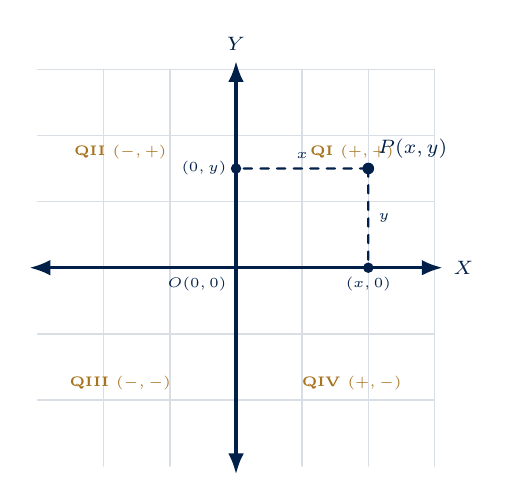
\begin{tikzpicture}[scale=1.05, line cap=round, line join=round]
  % Grid
  \draw[primary!15, line width=0.5pt, step=0.8cm] (-2.4,-2.4) grid (2.4,2.4);

  % Axes
  \draw[{Latex[scale=0.9]}-{Latex[scale=0.9]}, primary, line width=1.2pt] (-2.5,0) -- (2.5,0) node[right, font=\scriptsize\bfseries]{$X$};
  \draw[{Latex[scale=0.9]}-{Latex[scale=0.9]}, primary, line width=1.2pt] (0,-2.5) -- (0,2.5) node[above, font=\scriptsize\bfseries]{$Y$};
  \node[font=\tiny\bfseries\color{navy}, below left] at (0,0) {$O(0,0)$};

  % Quadrants
  \node[font=\tiny\bfseries\color{accent!80!black}] at (1.4,1.4) {QI $(+,+)$};
  \node[font=\tiny\bfseries\color{accent!80!black}] at (-1.4,1.4) {QII $(-,+)$};
  \node[font=\tiny\bfseries\color{accent!80!black}] at (-1.4,-1.4) {QIII $(-,-)$};
  \node[font=\tiny\bfseries\color{accent!80!black}] at (1.4,-1.4) {QIV $(+,-)$};

  % Point P(x,y)
  \coordinate (P) at (1.6,1.2);
  \fill[reddeep] (P) circle (2pt) node[above right, font=\scriptsize\bfseries\color{reddeep}]{$P(x,y)$};
  \draw[dashed, reddeep, line width=0.8pt] (P) -- (1.6,0) node[midway, right, font=\tiny\bfseries]{$y$};
  \draw[dashed, reddeep, line width=0.8pt] (P) -- (0,1.2) node[midway, above, font=\tiny\bfseries]{$x$};

  % Axis Points
  \fill[primary] (1.6,0) circle (1.8pt) node[below, font=\tiny\bfseries]{$(x,0)$};
  \fill[primary] (0,1.2) circle (1.8pt) node[left, font=\tiny\bfseries]{$(0,y)$};
\end{tikzpicture}
\end{minipage}\hfill
\begin{minipage}[c]{0.53\textwidth}
\begin{formulaBox}
  \textbf{Fundamental Anatomy of an Ordered Pair $(x,y)$:}
  \begin{itemize}
    \item \textbf{Abscissa ($x$-coordinate):} The signed horizontal distance of point $P$ from the vertical $y$-axis.
    \item \textbf{Ordinate ($y$-coordinate):} The signed vertical distance of point $P$ from the horizontal $x$-axis.
    \item \textbf{Points on Coordinate Axes:}
      \begin{itemize}
        \item Any point on the \textbf{$x$-axis} has ordinate zero: $\mathbf{(x, 0)}$.
        \item Any point on the \textbf{$y$-axis} has abscissa zero: $\mathbf{(0, y)}$.
      \end{itemize}
    \item \textbf{Distance of $P(x,y)$ from Coordinate Axes:}
      $$\mathbf{\text{Distance of } P(x,y) \text{ from } x\text{-axis}} = |y| = |\text{ordinate}|$$
      $$\mathbf{\text{Distance of } P(x,y) \text{ from } y\text{-axis}} = |x| = |\text{abscissa}|$$
  \end{itemize}
\end{formulaBox}
\end{minipage}

\vspace{0.8mm}
\subhead{1.2 The Absolute Value Distance Axiom}

\begin{warningBox}
  \textbf{\TrapTag\ Distance is Always Non-Negative!}
  Coordinates can be negative, but geometric distance is \textbf{strictly non-negative}:
  \begin{itemize}
    \item The distance of the point $P(-4, -7)$ from the $x$-axis is \textbf{$|-7| = 7\text{ units}$}, NOT $-7$.
    \item The distance of the point $P(-4, -7)$ from the $y$-axis is \textbf{$|-4| = 4\text{ units}$}, NOT $-4$.
    \item In CBSE MCQs, examiners frequently include negative options to trap students who forget absolute values.
  \end{itemize}
\end{warningBox}

\vspace{0.8mm}
\begin{conceptBox}[title={Worked Archetype 1 $\vert$ Axis Projections and Distance Identification},fonttitle=\bfseries\color{navy}]
  \textbf{Problem:} (i) Write the coordinates of the foot of the perpendicular drawn from $P(-5, 8)$ to the $y$-axis. (ii) What is the distance of $P$ from the $x$-axis? (iii) In which quadrant does $Q(a, b)$ lie if $a < 0$ and $b > 0$?
  \par\vspace{0.6mm}\noindent
  \textbf{Solution:}
  \begin{enumerate}
    \item The foot of the perpendicular from $P(-5, 8)$ to the $y$-axis lies directly on the $y$-axis, sharing the same $y$-coordinate. Hence, its coordinates are $\mathbf{(0, 8)}$.
    \item Distance of $P(-5, 8)$ from the $x$-axis $= |y| = |8| = \mathbf{8\text{ units}}$.
    \item For $Q(a, b)$, since abscissa $a < 0$ (negative) and ordinate $b > 0$ (positive), point $Q$ lies in \textbf{Quadrant II (QII)}.
  \end{enumerate}
\end{conceptBox}

\newpage

% =============================================================================
% PAGE 3: MODULE 2 — THE DISTANCE FORMULA & GEOMETRIC PROOF
% =============================================================================
\thispagestyle{fancy}
\vspace*{0mm}

\chapterbanner{07}{COORDINATE GEOMETRY}{Module 2 $\vert$ The Distance Formula: Pythagorean Derivation \& Origin Projections}{\CoreTag}

\subhead{2.1 Geometric Proof via the Pythagorean Theorem}

Let $P(x_1, y_1)$ and $Q(x_2, y_2)$ be any two points in the Cartesian plane. Draw $PR$ and $QS$ perpendicular to the $x$-axis, and draw $PT$ perpendicular to $QS$.

\begin{minipage}[c]{0.45\textwidth}
\centering
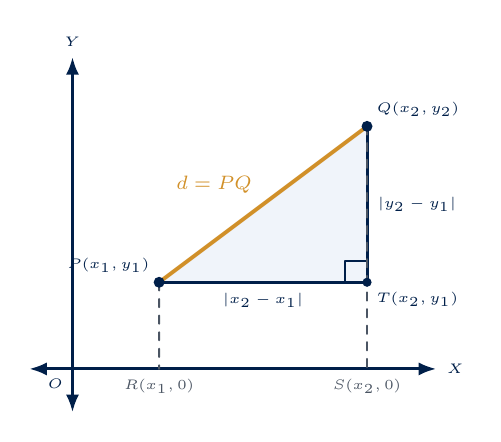
\begin{tikzpicture}[scale=1.1, line cap=round, line join=round]
  % Axes
  \draw[{Latex[scale=0.8]}-{Latex[scale=0.8]}, primary, line width=1.1pt] (-0.5,0) -- (4.2,0) node[right, font=\tiny\bfseries]{$X$};
  \draw[{Latex[scale=0.8]}-{Latex[scale=0.8]}, primary, line width=1.1pt] (0,-0.5) -- (0,3.6) node[above, font=\tiny\bfseries]{$Y$};
  \node[font=\tiny\bfseries\color{navy}, below left] at (0,0) {$O$};

  % Points
  \coordinate (P) at (1.0,1.0);
  \coordinate (Q) at (3.4,2.8);
  \coordinate (T) at (3.4,1.0);

  % Shaded right triangle
  \fill[primarylight] (P) -- (T) -- (Q) -- cycle;
  \draw[primary, line width=1.1pt] (P) -- (T) node[midway, below, font=\tiny\bfseries\color{navy}]{$|x_2 - x_1|$};
  \draw[primary, line width=1.1pt] (T) -- (Q) node[midway, right, font=\tiny\bfseries\color{navy}]{$|y_2 - y_1|$};
  \draw[accent, line width=1.4pt] (P) -- (Q) node[midway, above left, font=\scriptsize\bfseries\color{accent}]{$d = PQ$};

  % Right angle mark at T
  \draw[reddeep, line width=0.7pt] (3.15,1.0) -- (3.15,1.25) -- (3.4,1.25);

  % Drop lines to x-axis
  \draw[dashed, secondary, line width=0.7pt] (P) -- (1.0,0) node[below, font=\tiny\bfseries]{$R(x_1,0)$};
  \draw[dashed, secondary, line width=0.7pt] (Q) -- (3.4,0) node[below, font=\tiny\bfseries]{$S(x_2,0)$};

  \fill[reddeep] (P) circle (1.8pt) node[above left, font=\tiny\bfseries\color{reddeep}]{$P(x_1,y_1)$};
  \fill[reddeep] (Q) circle (1.8pt) node[above right, font=\tiny\bfseries\color{reddeep}]{$Q(x_2,y_2)$};
  \fill[primary] (T) circle (1.5pt) node[below right, font=\tiny\bfseries]{$T(x_2,y_1)$};
\end{tikzpicture}
\end{minipage}\hfill
\begin{minipage}[c]{0.53\textwidth}
\begin{formulaBox}
  \textbf{Step-by-Step Derivation:}
  \begin{enumerate}
    \item Horizontal projection: $PT = RS = OS - OR = x_2 - x_1$.
    \item Vertical projection: $QT = QS - TS = QS - PR = y_2 - y_1$.
    \item In right-angled triangle $\triangle PTQ$, by Pythagoras Theorem:
      $$PQ^2 = PT^2 + QT^2$$
      $$PQ^2 = (x_2 - x_1)^2 + (y_2 - y_1)^2$$
    \item Taking the positive square root (since distance $\ge 0$):
      $$\mathbf{d = \sqrt{(x_2 - x_1)^2 + (y_2 - y_1)^2}}$$
  \end{enumerate}
\end{formulaBox}
\end{minipage}

\vspace{0.8mm}
\subhead{2.2 Symmetry Properties \& Distance from the Origin}

\begin{formulaBox}
  \textbf{Essential Operational Invariants:}
  \begin{itemize}
    \item \textbf{Symmetry of Direction:} Since $(a - b)^2 = (b - a)^2$, the order of points is completely irrelevant:
      $$\mathbf{d = \sqrt{(x_2 - x_1)^2 + (y_2 - y_1)^2} = \sqrt{(x_1 - x_2)^2 + (y_1 - y_2)^2}}$$
    \item \textbf{Distance of Any Point $P(x,y)$ from the Origin $O(0,0)$:}
      $$\mathbf{OP = \sqrt{(x - 0)^2 + (y - 0)^2} = \sqrt{x^2 + y^2}}$$
  \end{itemize}
\end{formulaBox}

\vspace{0.8mm}
\begin{conceptBox}[title={Worked Archetype 2 $\vert$ Evaluating Distance with Radical and Negative Coordinates},fonttitle=\bfseries\color{navy}]
  \textbf{Problem:} Find the distance between: (i) $P(-6, 7)$ and $Q(-1, -5)$, and (ii) $A(a\cos\theta, 0)$ and $B(0, a\sin\theta)$.
  \par\vspace{0.6mm}\noindent
  \textbf{Solution (i):} Here $(x_1, y_1) = (-6, 7)$ and $(x_2, y_2) = (-1, -5)$.
  $$PQ = \sqrt{[-1 - (-6)]^2 + [-5 - 7]^2} = \sqrt{(-1 + 6)^2 + (-12)^2} = \sqrt{5^2 + (-12)^2} = \sqrt{25 + 144} = \sqrt{169} = \mathbf{13\text{ units.}}$$
  \textbf{Solution (ii):}
  $$AB = \sqrt{(0 - a\cos\theta)^2 + (a\sin\theta - 0)^2} = \sqrt{a^2\cos^2\theta + a^2\sin^2\theta} = \sqrt{a^2(\cos^2\theta + \sin^2\theta)} = \sqrt{a^2(1)} = \mathbf{|a|\text{ units.}}$$
\end{conceptBox}

\newpage

% =============================================================================
% PAGE 4: MODULE 3 — COLLINEARITY & THE 4-WAY TRIANGLE CLASSIFIER
% =============================================================================
\thispagestyle{fancy}
\vspace*{0mm}

\chapterbanner{07}{COORDINATE GEOMETRY}{Module 3 $\vert$ Collinearity \& Geometric Triangle Classification}{\CoreTag}

\subhead{3.1 Testing Collinearity Without the Area Formula}

Under the rationalized CBSE 2026--27 curriculum, the area of a triangle formula is deleted. Collinearity of three points $A, B, C$ must be established using the \textbf{Distance Sum Property}:

\begin{minipage}[c]{0.45\textwidth}
\centering
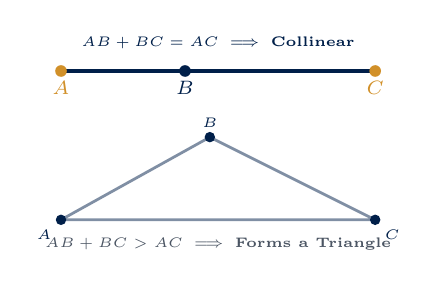
\begin{tikzpicture}[scale=1.05, line cap=round, line join=round]
  % Collinear line
  \draw[primary, line width=1.3pt] (0,1.8) -- (3.8,1.8);
  \fill[accent] (0,1.8) circle (2pt) node[below, font=\scriptsize\bfseries\color{navy}]{$A$};
  \fill[reddeep] (1.5,1.8) circle (2pt) node[below, font=\scriptsize\bfseries\color{reddeep}]{$B$};
  \fill[accent] (3.8,1.8) circle (2pt) node[below, font=\scriptsize\bfseries\color{navy}]{$C$};
  \node[font=\tiny\bfseries\color{navy}, above] at (1.9,1.95) {$AB + BC = AC \implies \text{Collinear}$};

  % Non-collinear triangle
  \draw[primary!50, line width=1pt] (0,0) -- (3.8,0) -- (1.8,1.0) -- cycle;
  \fill[primary] (0,0) circle (1.8pt) node[below left, font=\tiny\bfseries]{$A$};
  \fill[primary] (3.8,0) circle (1.8pt) node[below right, font=\tiny\bfseries]{$C$};
  \fill[reddeep] (1.8,1.0) circle (1.8pt) node[above, font=\tiny\bfseries\color{reddeep}]{$B$};
  \node[font=\tiny\bfseries\color{secondary}, below] at (1.9,-0.1) {$AB + BC > AC \implies \text{Forms a Triangle}$};
\end{tikzpicture}
\end{minipage}\hfill
\begin{minipage}[c]{0.53\textwidth}
\begin{formulaBox}
  \textbf{The Collinearity Criterion:}
  Three distinct points $A, B$, and $C$ are \textbf{collinear} (lie on the same straight line) if and only if:
  $$\mathbf{\text{Sum of two smaller distances} = \text{The largest distance}}$$
  That is, one of the following holds:
  \begin{itemize}
    \item $AB + BC = AC \iff B$ lies between $A$ and $C$.
    \item $AB + AC = BC \iff A$ lies between $B$ and $C$.
    \item $BC + AC = AB \iff C$ lies between $A$ and $B$.
  \end{itemize}
  \textit{If the sum of any two is strictly greater than the third, they form a non-degenerate triangle.}
\end{formulaBox}
\end{minipage}

\vspace{0.8mm}
\subhead{3.2 The 4-Way Triangle Classifier (Sides \& Angles)}

To determine the nature of a triangle formed by three given vertices $A, B, C$:
\begin{enumerate}
  \item Compute the three side lengths: $a = BC$, $b = CA$, and $c = AB$ using the distance formula.
  \item Apply the classification criteria below:
\end{enumerate}

\begin{center}
\small
\begin{tabularx}{\textwidth}{>{\bfseries}p{34mm} p{38mm} X}
\toprule
\rowcolor{bluepale}
\textbf{Triangle Type} & \textbf{Geometric Condition} & \textbf{Computational Check via Distance Formula} \\
\midrule
\textbf{Equilateral Triangle} & All 3 sides are equal & $AB = BC = CA$ \\
\rowcolor{lightgray}
\textbf{Isosceles Triangle} & Any 2 sides are equal & $AB = BC \neq CA$ (or any two equal) \\
\textbf{Scalene Triangle} & All 3 sides are unequal & $AB \neq BC \neq CA$ \\
\rowcolor{lightgray}
\textbf{Right-Angled Triangle} & Satisfies Pythagoras Converse & $(\text{Smallest side})^2 + (\text{Middle side})^2 = (\text{Largest side})^2$ \\
\textbf{Isosceles Right $\triangle$} & 2 sides equal + Pythagoras & $a^2 + a^2 = c^2 \iff 2a^2 = c^2$ where $c$ is hypotenuse \\
\bottomrule
\end{tabularx}
\end{center}

\vspace{0.5mm}
\begin{conceptBox}[title={Worked Archetype 3 $\vert$ Proving an Isosceles Right-Angled Triangle},fonttitle=\bfseries\color{navy}]
  \textbf{Problem:} Show that the points $A(3, 0)$, $B(6, 4)$, and $C(-1, 3)$ are the vertices of a right-angled isosceles triangle.
  \par\vspace{0.6mm}\noindent
  \textbf{Step 1: Compute the squares of the three side lengths to avoid premature square roots:}
  $$AB^2 = (6 - 3)^2 + (4 - 0)^2 = 3^2 + 4^2 = 9 + 16 = \mathbf{25} \implies AB = 5$$
  $$BC^2 = (-1 - 6)^2 + (3 - 4)^2 = (-7)^2 + (-1)^2 = 49 + 1 = \mathbf{50} \implies BC = \sqrt{50} = 5\sqrt{2}$$
  $$CA^2 = (3 - (-1))^2 + (0 - 3)^2 = 4^2 + (-3)^2 = 16 + 9 = \mathbf{25} \implies CA = 5$$
  \textbf{Step 2: Check side equality:} $AB = CA = 5 \implies \triangle ABC$ is \textbf{isosceles}.\\
  \textbf{Step 3: Check Pythagoras Converse:} $AB^2 + CA^2 = 25 + 25 = 50 = BC^2 \implies \angle A = 90^\circ$.\\
  Hence, $\triangle ABC$ is an \textbf{isosceles right-angled triangle} with hypotenuse $BC$.
\end{conceptBox}

\newpage

% =============================================================================
% PAGE 5: MODULE 4 — QUADRILATERAL IDENTIFICATION HIERARCHY
% =============================================================================
\thispagestyle{fancy}
\vspace*{0mm}

\chapterbanner{07}{COORDINATE GEOMETRY}{Module 4 $\vert$ Quadrilateral Identification: The 2-Tier Diagnostic Hierarchy}{\CoreTag}

\subhead{4.1 The 2-Tier Diagnostic Protocol for Four Given Vertices}

To rigorously identify the exact geometrical nature of a quadrilateral $ABCD$ given four vertices in cyclic order, \textbf{evaluating side lengths alone is never sufficient}. You must execute the 2-Tier Protocol:

\begin{center}
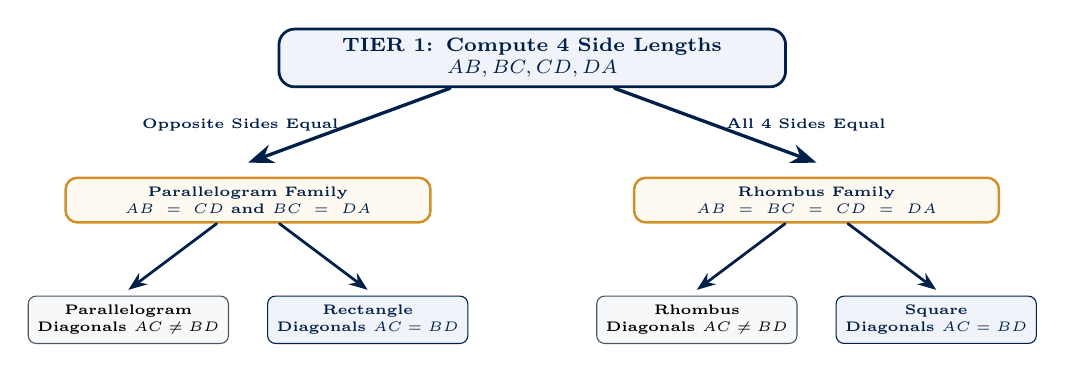
\begin{tikzpicture}[scale=0.95, line cap=round, line join=round]
  % Tier 1 Box
  \node[draw=primary, fill=primarylight, rounded corners=2mm, line width=1pt, font=\scriptsize\bfseries\color{navy}, align=center, text width=6.2cm] (T1) at (0,2.6) {\textbf{TIER 1: Compute 4 Side Lengths}\\$AB, BC, CD, DA$};

  % Split arrows
  \draw[-{Stealth[scale=1.1]}, primary, line width=1.2pt] (T1) -- (-3.8,1.2) node[midway, left, font=\tiny\bfseries]{Opposite Sides Equal};
  \draw[-{Stealth[scale=1.1]}, primary, line width=1.2pt] (T1) -- (3.8,1.2) node[midway, right, font=\tiny\bfseries]{All 4 Sides Equal};

  % Branch A: Parallelogram family
  \node[draw=accent, fill=accentlight, rounded corners=1.5mm, line width=0.9pt, font=\tiny\bfseries\color{navy}, align=center, text width=4.4cm] (B1) at (-3.8,0.7) {\textbf{Parallelogram Family}\\$AB = CD$ and $BC = DA$};

  % Branch B: Rhombus family
  \node[draw=accent, fill=accentlight, rounded corners=1.5mm, line width=0.9pt, font=\tiny\bfseries\color{navy}, align=center, text width=4.4cm] (B2) at (3.8,0.7) {\textbf{Rhombus Family}\\$AB = BC = CD = DA$};

  % Tier 2 diagonal checks
  \draw[-{Stealth[scale=0.9]}, reddeep, line width=1pt] (B1) -- (-5.4,-0.5);
  \draw[-{Stealth[scale=0.9]}, green, line width=1pt] (B1) -- (-2.2,-0.5);

  \draw[-{Stealth[scale=0.9]}, reddeep, line width=1pt] (B2) -- (2.2,-0.5);
  \draw[-{Stealth[scale=0.9]}, green, line width=1pt] (B2) -- (5.4,-0.5);

  % Leaves
  \node[draw=secondary, fill=lightgray, rounded corners=1mm, font=\tiny\bfseries, align=center] at (-5.4,-0.9) {\textbf{Parallelogram}\\Diagonals $AC \neq BD$};
  \node[draw=green, fill=greenpale, rounded corners=1mm, font=\tiny\bfseries\color{green}, align=center] at (-2.2,-0.9) {\textbf{Rectangle}\\Diagonals $AC = BD$};
  \node[draw=secondary, fill=lightgray, rounded corners=1mm, font=\tiny\bfseries, align=center] at (2.2,-0.9) {\textbf{Rhombus}\\Diagonals $AC \neq BD$};
  \node[draw=green, fill=greenpale, rounded corners=1mm, font=\tiny\bfseries\color{green}, align=center] at (5.4,-0.9) {\textbf{Square}\\Diagonals $AC = BD$};
\end{tikzpicture}
\end{center}

\vspace{0.8mm}
\subhead{4.2 The Complete 6-Distance Verification Matrix}

\begin{center}
\small
\begin{tabularx}{\textwidth}{p{32mm} p{48mm} p{36mm} X}
\toprule
\rowcolor{bluepale}
\textbf{Quadrilateral} & \textbf{Tier 1: Side Length Conditions} & \textbf{Tier 2: Diagonal Conditions} & \textbf{CBSE Board Verdict} \\
\midrule
\textbf{Parallelogram} & $AB = CD$ and $BC = DA$ & $AC \neq BD$ & Diagonals unequal $\implies$ not a rectangle. \\
\rowcolor{lightgray}
\textbf{Rectangle} & $AB = CD$ and $BC = DA$ & $\mathbf{AC = BD}$ & Equal diagonals prove right angles. \\
\textbf{Rhombus} & $AB = BC = CD = DA$ & $AC \neq BD$ & Unequal diagonals $\implies$ not a square. \\
\rowcolor{lightgray}
\textbf{Square} & $AB = BC = CD = DA$ & $\mathbf{AC = BD}$ & Equal diagonals prove all angles $90^\circ$. \\
\bottomrule
\end{tabularx}
\end{center}

\vspace{0.5mm}
\begin{conceptBox}[title={Worked Archetype 4 $\vert$ Proving Four Points Form a Rhombus but Not a Square},fonttitle=\bfseries\color{navy}]
  \textbf{Problem:} Show that $A(3, 0)$, $B(4, 5)$, $C(-1, 4)$, and $D(-2, -1)$ are the vertices of a rhombus. Is it a square?
  \par\vspace{0.6mm}\noindent
  \textbf{Tier 1: Calculate the 4 side lengths:}
  \begin{itemize}
    \item $AB^2 = (4 - 3)^2 + (5 - 0)^2 = 1^2 + 5^2 = 26 \implies AB = \sqrt{26}$
    \item $BC^2 = (-1 - 4)^2 + (4 - 5)^2 = (-5)^2 + (-1)^2 = 26 \implies BC = \sqrt{26}$
    \item $CD^2 = [-2 - (-1)]^2 + (-1 - 4)^2 = (-1)^2 + (-5)^2 = 26 \implies CD = \sqrt{26}$
    \item $DA^2 = [3 - (-2)]^2 + [0 - (-1)]^2 = 5^2 + 1^2 = 26 \implies DA = \sqrt{26}$
  \end{itemize}
  Since $AB = BC = CD = DA = \sqrt{26}$, the quadrilateral $ABCD$ is a \textbf{rhombus}.
  \par\noindent
  \textbf{Tier 2: Calculate the 2 diagonal lengths:}
  \begin{itemize}
    \item $AC^2 = (-1 - 3)^2 + (4 - 0)^2 = (-4)^2 + 4^2 = 16 + 16 = 32 \implies AC = \sqrt{32} = 4\sqrt{2}$
    \item $BD^2 = (-2 - 4)^2 + (-1 - 5)^2 = (-6)^2 + (-6)^2 = 36 + 36 = 72 \implies BD = \sqrt{72} = 6\sqrt{2}$
  \end{itemize}
  Since diagonals $\mathbf{AC \neq BD}$, the internal angles are not right angles. Hence, $ABCD$ is \textbf{a rhombus, but NOT a square}.
\end{conceptBox}

\newpage

% =============================================================================
% PAGE 6: MODULE 5 — EQUIDISTANT POINTS & LOCUS PROBLEMS
% =============================================================================
\thispagestyle{fancy}
\vspace*{0mm}

\chapterbanner{07}{COORDINATE GEOMETRY}{Module 5 $\vert$ Equidistant Points, Perpendicular Bisectors \& Locus}{\CoreTag}

\subhead{5.1 The Equidistance Principle: $PA = PB \iff PA^2 = PB^2$}

A point $P$ is equidistant from two fixed points $A$ and $B$ if the straight-line distances $PA$ and $PB$ are identical.
\begin{itemize}
  \item \textbf{Computational Golden Rule:} Always equate the squares of the distances: $\mathbf{PA^2 = PB^2}$. This eliminates square roots immediately, preventing arithmetic errors.
\end{itemize}

\begin{minipage}[c]{0.45\textwidth}
\centering
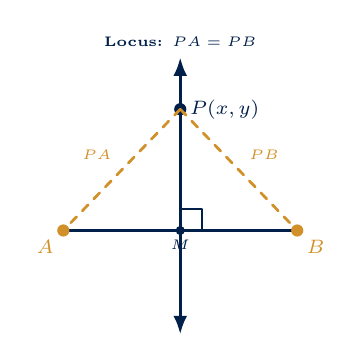
\begin{tikzpicture}[scale=1.1, line cap=round, line join=round]
  % Fixed points A and B
  \coordinate (A) at (0.5,0.6);
  \coordinate (B) at (3.2,0.6);
  \draw[primary, line width=1.1pt] (A) -- (B);
  \fill[accent] (A) circle (2pt) node[below left, font=\scriptsize\bfseries\color{navy}]{$A$};
  \fill[accent] (B) circle (2pt) node[below right, font=\scriptsize\bfseries\color{navy}]{$B$};

  % Midpoint M
  \coordinate (M) at (1.85,0.6);
  \fill[primary] (M) circle (1.5pt) node[below, font=\tiny\bfseries]{$M$};

  % Perpendicular bisector locus line
  \draw[{Latex[scale=0.8]}-{Latex[scale=0.8]}, reddeep, line width=1.2pt] (1.85,-0.6) -- (1.85,2.6) node[above, font=\tiny\bfseries\color{reddeep}]{Locus: $PA = PB$};

  % Point P on locus
  \coordinate (P) at (1.85,2.0);
  \fill[reddeep] (P) circle (2pt) node[right, font=\scriptsize\bfseries\color{reddeep}]{$P(x,y)$};
  \draw[dashed, accent, line width=1pt] (P) -- (A) node[midway, above left, font=\tiny\bfseries\color{accent}]{$PA$};
  \draw[dashed, accent, line width=1pt] (P) -- (B) node[midway, above right, font=\tiny\bfseries\color{accent}]{$PB$};

  % Right angle at M
  \draw[reddeep, line width=0.6pt] (1.85,0.85) -- (2.1,0.85) -- (2.1,0.6);
\end{tikzpicture}
\end{minipage}\hfill
\begin{minipage}[c]{0.53\textwidth}
\begin{formulaBox}
  \textbf{Equidistant Point Configurations on Coordinate Axes:}
  \begin{itemize}
    \item \textbf{Point on the $x$-axis:}
      $$\text{Assume } \mathbf{P(x, 0)} \implies PA^2 = PB^2$$
      Solves for a single unknown $x$.
    \item \textbf{Point on the $y$-axis:}
      $$\text{Assume } \mathbf{P(0, y)} \implies PA^2 = PB^2$$
      Solves for a single unknown $y$.
    \item \textbf{Geometric Locus (Perpendicular Bisector):}
      The collection of all points $P(x,y)$ equidistant from $A$ and $B$ forms a straight line. Expanding $PA^2 = PB^2$ always causes the quadratic terms ($x^2, y^2$) to cancel out, leaving a \textbf{linear equation} $Ax + By + C = 0$.
  \end{itemize}
\end{formulaBox}
\end{minipage}

\vspace{0.8mm}
\begin{conceptBox}[title={Worked Archetype 5 $\vert$ Finding a Point on the $x$-axis Equidistant from Two Points},fonttitle=\bfseries\color{navy}]
  \textbf{Problem:} Find the point on the $x$-axis which is equidistant from $A(2, -5)$ and $B(-2, 9)$.
  \par\vspace{0.6mm}\noindent
  \textbf{Step 1: Define point on $x$-axis:} Since the point lies on the $x$-axis, its ordinate is zero. Let $P(x, 0)$.\\
  \textbf{Step 2: Apply the equidistance condition:} $PA = PB \iff PA^2 = PB^2$.
  $$(x - 2)^2 + [0 - (-5)]^2 = [x - (-2)]^2 + (0 - 9)^2$$
  $$(x - 2)^2 + 5^2 = (x + 2)^2 + (-9)^2$$
  \textbf{Step 3: Expand and cancel quadratic terms:}
  $$x^2 - 4x + 4 + 25 = x^2 + 4x + 4 + 81$$
  $$-4x + 29 = 4x + 85 \implies -8x = 85 - 29 = 56 \implies x = \frac{56}{-8} = \mathbf{-7}$$
  \textbf{Conclusion:} The required point on the $x$-axis is $\mathbf{P(-7, 0)}$.
\end{conceptBox}

\vspace{0.8mm}
\begin{conceptBox}[title={Worked Archetype 6 $\vert$ Linear Relation between $x$ and $y$ (Perpendicular Bisector)},fonttitle=\bfseries\color{navy}]
  \textbf{Problem:} Find a relation between $x$ and $y$ such that the point $P(x, y)$ is equidistant from $A(3, 6)$ and $B(-3, 4)$.
  \par\vspace{0.6mm}\noindent
  $$PA^2 = PB^2 \implies (x - 3)^2 + (y - 6)^2 = [x - (-3)]^2 + (y - 4)^2$$
  $$(x^2 - 6x + 9) + (y^2 - 12y + 36) = (x^2 + 6x + 9) + (y^2 - 8y + 16)$$
  $$-6x - 12y + 45 = 6x - 8y + 25$$
  $$-12x - 4y + 20 = 0 \implies \text{Divide by } -4: \quad \mathbf{3x + y - 5 = 0}$$
\end{conceptBox}

\newpage

% =============================================================================
% PAGE 7: MODULE 6 — THE SECTION FORMULA (INTERNAL DIVISION)
% =============================================================================
\thispagestyle{fancy}
\vspace*{0mm}

\chapterbanner{07}{COORDINATE GEOMETRY}{Module 6 $\vert$ The Section Formula: Similar Triangles Proof \& Midpoint Axiom}{\CoreTag}

\subhead{6.1 Geometric Derivation of the Section Formula}

Let $P(x,y)$ divide the line segment joining $A(x_1, y_1)$ and $B(x_2, y_2)$ internally in the ratio $m_1 : m_2$. Draw vertical lines from $A, P, B$ to the $x$-axis, and draw horizontal segments $AQ$ and $PC$.

\begin{minipage}[c]{0.45\textwidth}
\centering
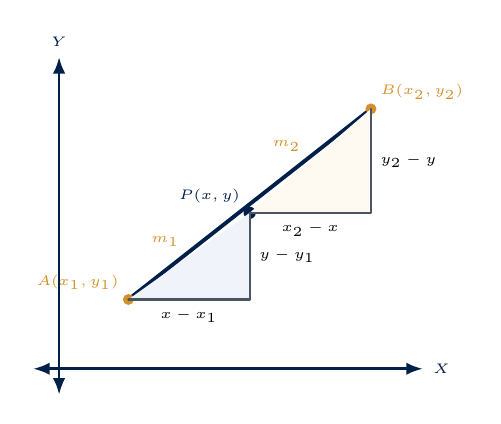
\begin{tikzpicture}[scale=1.1, line cap=round, line join=round]
  % Axes
  \draw[{Latex[scale=0.8]}-{Latex[scale=0.8]}, primary, line width=1pt] (-0.3,0) -- (4.2,0) node[right, font=\tiny\bfseries]{$X$};
  \draw[{Latex[scale=0.8]}-{Latex[scale=0.8]}, primary, line width=1pt] (0,-0.3) -- (0,3.6) node[above, font=\tiny\bfseries]{$Y$};

  % Points
  \coordinate (A) at (0.8,0.8);
  \coordinate (P) at (2.2,1.8);
  \coordinate (B) at (3.6,3.0);

  % Line AB
  \draw[primary, line width=1.4pt] (A) -- (B);
  \fill[accent] (A) circle (1.8pt) node[above left, font=\tiny\bfseries\color{navy}]{$A(x_1,y_1)$};
  \fill[reddeep] (P) circle (2pt) node[above left, font=\tiny\bfseries\color{reddeep}]{$P(x,y)$};
  \fill[accent] (B) circle (1.8pt) node[above right, font=\tiny\bfseries\color{navy}]{$B(x_2,y_2)$};

  % Similar triangles
  \coordinate (Q) at (2.2,0.8);
  \coordinate (C) at (3.6,1.8);
  \fill[primarylight] (A) -- (Q) -- (P) -- cycle;
  \fill[accentlight] (P) -- (C) -- (B) -- cycle;
  \draw[secondary, line width=0.8pt] (A) -- (Q) -- (P);
  \draw[secondary, line width=0.8pt] (P) -- (C) -- (B);

  % Ratio markings
  \node[font=\tiny\bfseries\color{accent}, above left] at (1.5,1.3) {$m_1$};
  \node[font=\tiny\bfseries\color{accent}, above left] at (2.9,2.4) {$m_2$};

  % Displacements
  \node[font=\tiny\bfseries, below] at (1.5,0.8) {$x - x_1$};
  \node[font=\tiny\bfseries, right] at (2.2,1.3) {$y - y_1$};
  \node[font=\tiny\bfseries, below] at (2.9,1.8) {$x_2 - x$};
  \node[font=\tiny\bfseries, right] at (3.6,2.4) {$y_2 - y$};
\end{tikzpicture}
\end{minipage}\hfill
\begin{minipage}[c]{0.53\textwidth}
\begin{formulaBox}
  \textbf{Similar Triangles Step-by-Step Proof:}
  In $\triangle AQP$ and $\triangle PCB$, since the corresponding angles are equal ($\angle A = \angle P$, right angles at $Q, C$):
  $$\triangle AQP \sim \triangle PCB \quad (\text{AA similarity})$$
  $$\frac{AQ}{PC} = \frac{QP}{CB} = \frac{AP}{PB} = \frac{m_1}{m_2}$$
  \textbf{Equating horizontal ratio:}
  $$\frac{x - x_1}{x_2 - x} = \frac{m_1}{m_2} \implies (m_1 + m_2)x = m_1 x_2 + m_2 x_1$$
  $$\mathbf{x = \frac{m_1 x_2 + m_2 x_1}{m_1 + m_2}}$$
  Similarly, equating vertical ratios yields:
  $$\mathbf{y = \frac{m_1 y_2 + m_2 y_1}{m_1 + m_2}}$$
\end{formulaBox}
\end{minipage}

\vspace{0.8mm}
\subhead{6.2 The Master Section Formula Suite \& The Midpoint Special Case}

\begin{formulaBox}
  \textbf{The Section Formula for Internal Division ($P$ divides $AB$ in ratio $m_1 : m_2$):}
  $$\mathbf{P(x, y) = \left( \frac{m_1 x_2 + m_2 x_1}{m_1 + m_2}, \; \frac{m_1 y_2 + m_2 y_1}{m_1 + m_2} \right)}$$
  \textbf{The Midpoint Formula ($1 : 1$ Division, where $m_1 = m_2 = 1$):}
  $$\mathbf{M(x, y) = \left( \frac{x_1 + x_2}{2}, \; \frac{y_1 + y_2}{2} \right)}$$
\end{formulaBox}

\vspace{0.8mm}
\begin{conceptBox}[title={Worked Archetype 7 $\vert$ Direct Application of Section and Midpoint Formulas},fonttitle=\bfseries\color{navy}]
  \textbf{Problem:} (i) Find coordinates of point $P$ dividing $A(4, -3)$ and $B(8, 5)$ in ratio $3 : 1$. (ii) Find midpoint $M$ of $AB$.
  \par\vspace{0.6mm}\noindent
  \textbf{Solution (i):} Here $(x_1, y_1) = (4, -3)$, $(x_2, y_2) = (8, 5)$, $m_1 = 3$, $m_2 = 1$.
  $$x = \frac{m_1 x_2 + m_2 x_1}{m_1 + m_2} = \frac{3(8) + 1(4)}{3 + 1} = \frac{24 + 4}{4} = \frac{28}{4} = \mathbf{7}$$
  $$y = \frac{m_1 y_2 + m_2 y_1}{m_1 + m_2} = \frac{3(5) + 1(-3)}{3 + 1} = \frac{15 - 3}{4} = \frac{12}{4} = \mathbf{3} \implies \mathbf{P(7, 3)}$$
  \textbf{Solution (ii):} $M = \left(\frac{4 + 8}{2}, \frac{-3 + 5}{2}\right) = \left(\frac{12}{2}, \frac{2}{2}\right) = \mathbf{(6, 1)}$.
\end{conceptBox}

\newpage

% =============================================================================
% PAGE 8: MODULE 7 — THE k : 1 RATIO PROTOCOL & AXIS INTERSECTIONS
% =============================================================================
\thispagestyle{fancy}
\vspace*{0mm}

\chapterbanner{07}{COORDINATE GEOMETRY}{Module 7 $\vert$ The $k : 1$ Ratio Parameterization \& Coordinate Axis Division}{\CoreTag}

\subhead{7.1 Why the $k : 1$ Method is Superior to $m_1 : m_2$}

When the dividing ratio is unknown, writing $m_1 : m_2$ introduces \textbf{two variables}, requiring system equations. Setting $\mathbf{k = \frac{m_1}{m_2}}$ reduces the problem to a \textbf{single unknown $k$}:
$$\mathbf{P(x, y) = \left( \frac{k x_2 + x_1}{k + 1}, \; \frac{k y_2 + y_1}{k + 1} \right)}$$
Once $k$ is found, the required ratio is $\mathbf{k : 1}$ (e.g., if $k = \frac{2}{3}$, ratio is $\frac{2}{3} : 1 \implies \mathbf{2 : 3}$).

\vspace{0.8mm}
\subhead{7.2 Division of a Line Segment by Coordinate Axes}

\begin{minipage}[c]{0.45\textwidth}
\centering
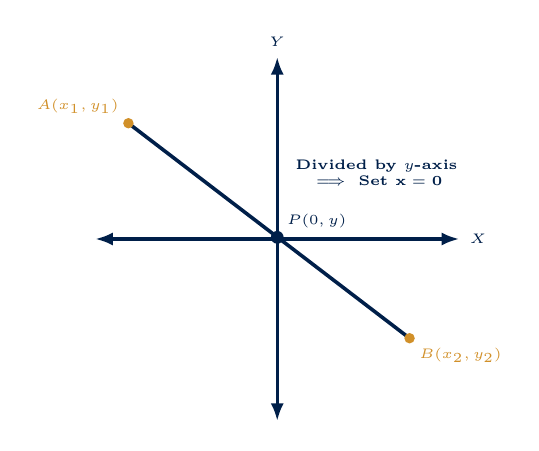
\begin{tikzpicture}[scale=1.05, line cap=round, line join=round]
  % Axes
  \draw[{Latex[scale=0.8]}-{Latex[scale=0.8]}, primary, line width=1.1pt] (-2.2,0) -- (2.2,0) node[right, font=\tiny\bfseries]{$X$};
  \draw[{Latex[scale=0.8]}-{Latex[scale=0.8]}, primary, line width=1.1pt] (0,-2.2) -- (0,2.2) node[above, font=\tiny\bfseries]{$Y$};

  % Segment intersecting Y-axis
  \coordinate (A) at (-1.8,1.4);
  \coordinate (B) at (1.6,-1.2);
  \draw[primary, line width=1.3pt] (A) -- (B);
  \fill[accent] (A) circle (1.8pt) node[above left, font=\tiny\bfseries\color{navy}]{$A(x_1,y_1)$};
  \fill[accent] (B) circle (1.8pt) node[below right, font=\tiny\bfseries\color{navy}]{$B(x_2,y_2)$};

  % Intersection point P(0, y)
  \coordinate (P) at (0,0.02);
  \fill[reddeep] (P) circle (2.2pt) node[above right, font=\tiny\bfseries\color{reddeep}]{$P(0, y)$};
  \node[font=\tiny\bfseries\color{reddeep}, align=center] at (1.2,0.8) {Divided by $y$-axis\\$\implies$ Set $\mathbf{x = 0}$};
\end{tikzpicture}
\end{minipage}\hfill
\begin{minipage}[c]{0.53\textwidth}
\begin{formulaBox}
  \textbf{The 2-Case Axis Intersection Rules:}
  \begin{itemize}
    \item \textbf{Case 1: Line Divided by the $x$-axis:}
      \begin{enumerate}
        \item Intersection point lies on $x$-axis: $\mathbf{P(x, 0)}$.
        \item Its $y$-coordinate is zero: set $\mathbf{\frac{k y_2 + y_1}{k + 1} = 0}$.
        \item Yields: $k y_2 + y_1 = 0 \implies \mathbf{k = -\frac{y_1}{y_2}}$.
      \end{enumerate}
    \item \textbf{Case 2: Line Divided by the $y$-axis:}
      \begin{enumerate}
        \item Intersection point lies on $y$-axis: $\mathbf{P(0, y)}$.
        \item Its $x$-coordinate is zero: set $\mathbf{\frac{k x_2 + x_1}{k + 1} = 0}$.
        \item Yields: $k x_2 + x_1 = 0 \implies \mathbf{k = -\frac{x_1}{x_2}}$.
      \end{enumerate}
  \end{itemize}
\end{formulaBox}
\end{minipage}

\vspace{0.8mm}
\begin{conceptBox}[title={Worked Archetype 8 $\vert$ Division of Line Segment by the $y$-axis},fonttitle=\bfseries\color{navy}]
  \textbf{Problem:} Find the ratio in which the $y$-axis divides the line segment joining the points $A(5, -6)$ and $B(-1, -4)$. Also find the point of intersection.
  \par\vspace{0.6mm}\noindent
  \textbf{Step 1: Set up the $k:1$ parameterization:} Let the $y$-axis divide $AB$ in the ratio $k : 1$ at point $P(0, y)$.
  $$P(x, y) = \left( \frac{k(-1) + 1(5)}{k + 1}, \; \frac{k(-4) + 1(-6)}{k + 1} \right) = \left( \frac{-k + 5}{k + 1}, \; \frac{-4k - 6}{k + 1} \right)$$
  \textbf{Step 2: Equate abscissa to zero:} Since $P$ lies on the $y$-axis, $x = 0$:
  $$\frac{-k + 5}{k + 1} = 0 \implies -k + 5 = 0 \implies \mathbf{k = 5}$$
  Thus, the required dividing ratio is $5 : 1 \implies \mathbf{5 : 1\text{ internally}}$.\\
  \textbf{Step 3: Find the $y$-coordinate of intersection:}
  $$y = \frac{-4(5) - 6}{5 + 1} = \frac{-20 - 6}{6} = \frac{-26}{6} = \mathbf{-\frac{13}{3}}$$
  \textbf{Conclusion:} The $y$-axis divides $AB$ in the ratio $\mathbf{5 : 1}$, and the point of intersection is $\mathbf{\left(0, -\frac{13}{3}\right)}$.
\end{conceptBox}

\newpage

% =============================================================================
% PAGE 9: MODULE 8 — POINTS OF TRISECTION & MULTI-SECTION MODELS
% =============================================================================
\thispagestyle{fancy}
\vspace*{0mm}

\chapterbanner{07}{COORDINATE GEOMETRY}{Module 8 $\vert$ Points of Trisection \& Multi-Segment Partitioning}{\CoreTag}

\subhead{8.1 The Geometry of Trisection Points}

The \textbf{points of trisection} of a line segment $AB$ are the two distinct points, say $P$ and $Q$, which divide the segment into three equal parts, such that $\mathbf{AP = PQ = QB}$.

\begin{center}
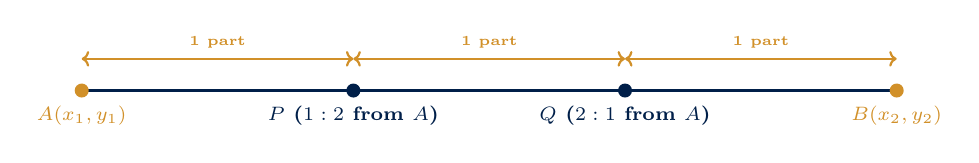
\begin{tikzpicture}[scale=1.15, line cap=round, line join=round]
  % Line AB
  \draw[primary, line width=1.4pt] (0,0) -- (9,0);

  % Ticks and points
  \fill[accent] (0,0) circle (2.2pt) node[below=2pt, font=\scriptsize\bfseries\color{navy}]{$A(x_1,y_1)$};
  \fill[reddeep] (3,0) circle (2.2pt) node[below=2pt, font=\scriptsize\bfseries\color{reddeep}]{$P$ ($1:2$ from $A$)};
  \fill[reddeep] (6,0) circle (2.2pt) node[below=2pt, font=\scriptsize\bfseries\color{reddeep}]{$Q$ ($2:1$ from $A$)};
  \fill[accent] (9,0) circle (2.2pt) node[below=2pt, font=\scriptsize\bfseries\color{navy}]{$B(x_2,y_2)$};

  % Brackets/Lengths
  \draw[{<[scale=0.8]}-{>[scale=0.8]}, accent, line width=0.8pt] (0,0.35) -- (3,0.35) node[midway, above, font=\tiny\bfseries]{1 part};
  \draw[{<[scale=0.8]}-{>[scale=0.8]}, accent, line width=0.8pt] (3,0.35) -- (6,0.35) node[midway, above, font=\tiny\bfseries]{1 part};
  \draw[{<[scale=0.8]}-{>[scale=0.8]}, accent, line width=0.8pt] (6,0.35) -- (9,0.35) node[midway, above, font=\tiny\bfseries]{1 part};
\end{tikzpicture}
\end{center}

\vspace{0.8mm}
\begin{formulaBox}
  \textbf{Master Ratios for Trisection Points:}
  \begin{itemize}
    \item \textbf{Point $P$:} Divides $AB$ internally in the ratio $\mathbf{1 : 2}$.
      $$\mathbf{P = \left( \frac{1(x_2) + 2(x_1)}{1 + 2}, \; \frac{1(y_2) + 2(y_1)}{1 + 2} \right) = \left( \frac{x_2 + 2x_1}{3}, \; \frac{y_2 + 2y_1}{3} \right)}$$
    \item \textbf{Point $Q$:} Divides $AB$ internally in the ratio $\mathbf{2 : 1}$.
      $$\mathbf{Q = \left( \frac{2(x_2) + 1(x_1)}{2 + 1}, \; \frac{2(y_2) + 1(y_1)}{2 + 1} \right) = \left( \frac{2x_2 + x_1}{3}, \; \frac{2y_2 + y_1}{3} \right)}$$
    \item \textbf{The High-Speed Midpoint Optimization:}
      Do NOT apply the full section formula twice! Once point $P$ is determined, observe that $Q$ is the \textbf{midpoint of segment $PB$}:
      $$\mathbf{Q = \text{Midpoint of } PB = \left(\frac{x_P + x_2}{2}, \; \frac{y_P + y_2}{2}\right)}$$
  \end{itemize}
\end{formulaBox}

\vspace{0.8mm}
\subhead{8.2 Partitioning into Four Equal Parts (Quadrisection)}

To divide a segment $AB$ into 4 equal segments:
\begin{enumerate}
  \item First, find the overall midpoint of $AB$, say $M = \left(\frac{x_1+x_2}{2}, \frac{y_1+y_2}{2}\right)$.
  \item Next, find the midpoint of $AM$, say $P_1$, and the midpoint of $MB$, say $P_2$.
\end{enumerate}

\vspace{0.8mm}
\begin{conceptBox}[title={Worked Archetype 9 $\vert$ Finding the Coordinates of the Points of Trisection},fonttitle=\bfseries\color{navy}]
  \textbf{Problem:} Find the coordinates of the points of trisection of the line segment joining $A(2, -2)$ and $B(-7, 4)$.
  \par\vspace{0.6mm}\noindent
  \textbf{Step 1: Point $P$ divides $AB$ in ratio $1 : 2$ ($m_1 = 1, m_2 = 2$):}
  $$x_P = \frac{1(-7) + 2(2)}{1 + 2} = \frac{-7 + 4}{3} = \frac{-3}{3} = \mathbf{-1}$$
  $$y_P = \frac{1(4) + 2(-2)}{1 + 2} = \frac{4 - 4}{3} = \frac{0}{3} = \mathbf{0} \implies \mathbf{P(-1, 0)}$$
  \textbf{Step 2: Use the Midpoint Optimization to find $Q$ (Midpoint of $PB$):}
  Here $P = (-1, 0)$ and $B = (-7, 4)$:
  $$x_Q = \frac{-1 + (-7)}{2} = \frac{-8}{2} = \mathbf{-4}$$
  $$y_Q = \frac{0 + 4}{2} = \frac{4}{2} = \mathbf{2} \implies \mathbf{Q(-4, 2)}$$
  \textbf{Conclusion:} The points of trisection are $\mathbf{P(-1, 0)}$ and $\mathbf{Q(-4, 2)}$.
\end{conceptBox}

\newpage

% =============================================================================
% PAGE 10: MODULE 9 — PARALLELOGRAM DIAGONAL TRICK & CENTROID OF A TRIANGLE
% =============================================================================
\thispagestyle{fancy}
\vspace*{0mm}

\chapterbanner{07}{COORDINATE GEOMETRY}{Module 9 $\vert$ The Parallelogram Diagonal Trick \& Centroid of a Triangle}{\CoreTag}

\subhead{9.1 The 10-Second Parallelogram Fourth-Vertex Technique}

In Euclidean geometry, \textbf{the diagonals of any parallelogram bisect each other}. Therefore, the diagonals $AC$ and $BD$ have the exact same midpoint $M$:

\begin{minipage}[c]{0.45\textwidth}
\centering
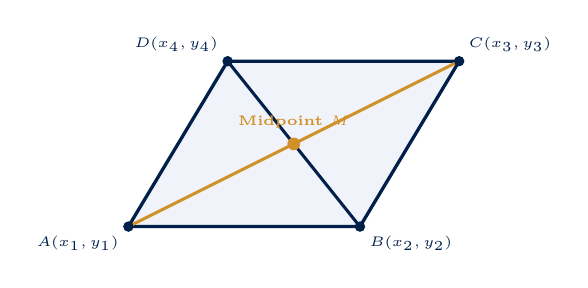
\begin{tikzpicture}[scale=1.05, line cap=round, line join=round]
  % Parallelogram ABCD
  \coordinate (A) at (0,0);
  \coordinate (B) at (2.8,0);
  \coordinate (C) at (4.0,2.0);
  \coordinate (D) at (1.2,2.0);

  \draw[primary, fill=primarylight, line width=1.2pt] (A) -- (B) -- (C) -- (D) -- cycle;

  % Diagonals
  \draw[accent, line width=1.1pt] (A) -- (C);
  \draw[reddeep, line width=1.1pt] (B) -- (D);

  % Common Midpoint M
  \coordinate (M) at (2.0,1.0);
  \fill[gold] (M) circle (2.2pt) node[above=2pt, font=\tiny\bfseries\color{navy}]{Midpoint $M$};

  \fill[primary] (A) circle (1.8pt) node[below left, font=\tiny\bfseries]{$A(x_1,y_1)$};
  \fill[primary] (B) circle (1.8pt) node[below right, font=\tiny\bfseries]{$B(x_2,y_2)$};
  \fill[primary] (C) circle (1.8pt) node[above right, font=\tiny\bfseries]{$C(x_3,y_3)$};
  \fill[primary] (D) circle (1.8pt) node[above left, font=\tiny\bfseries]{$D(x_4,y_4)$};
\end{tikzpicture}
\end{minipage}\hfill
\begin{minipage}[c]{0.53\textwidth}
\begin{formulaBox}
  \textbf{Algebraic Parallelogram Identity:}
  $$\text{Midpoint of } AC = \text{Midpoint of } BD$$
  $$\left( \frac{x_1 + x_3}{2}, \; \frac{y_1 + y_3}{2} \right) = \left( \frac{x_2 + x_4}{2}, \; \frac{y_2 + y_4}{2} \right)$$
  Equating coordinates yields the instantaneous formula:
  $$\mathbf{x_1 + x_3 = x_2 + x_4 \iff x_4 = x_1 + x_3 - x_2}$$
  $$\mathbf{y_1 + y_3 = y_2 + y_4 \iff y_4 = y_1 + y_3 - y_2}$$
  \textit{Avoids cumbersome distance formulas entirely!}
\end{formulaBox}
\end{minipage}

\vspace{0.8mm}
\subhead{9.2 Centroid of a Triangle (Center of Mass)}

The \textbf{centroid ($G$)} of a triangle is the point of intersection of its three medians. It divides every median internally in the ratio $\mathbf{2 : 1}$ (measured from vertex to base midpoint):

\begin{minipage}[c]{0.45\textwidth}
\centering
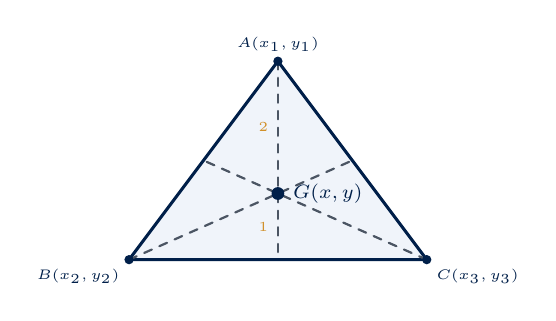
\begin{tikzpicture}[scale=1.05, line cap=round, line join=round]
  \coordinate (A) at (1.8,2.4);
  \coordinate (B) at (0,0);
  \coordinate (C) at (3.6,0);

  \draw[primary, fill=primarylight, line width=1.1pt] (A) -- (B) -- (C) -- cycle;

  % Midpoints
  \coordinate (D) at (1.8,0);
  \coordinate (E) at (2.7,1.2);
  \coordinate (F) at (0.9,1.2);

  % Medians
  \draw[dashed, secondary, line width=0.8pt] (A) -- (D);
  \draw[dashed, secondary, line width=0.8pt] (B) -- (E);
  \draw[dashed, secondary, line width=0.8pt] (C) -- (F);

  % Centroid G
  \coordinate (G) at (1.8,0.8);
  \fill[reddeep] (G) circle (2.2pt) node[right=2pt, font=\scriptsize\bfseries\color{reddeep}]{$G(x,y)$};
  \node[font=\tiny\bfseries\color{accent}, left] at (1.8,1.6) {$2$};
  \node[font=\tiny\bfseries\color{accent}, left] at (1.8,0.4) {$1$};

  \fill[primary] (A) circle (1.6pt) node[above, font=\tiny\bfseries]{$A(x_1,y_1)$};
  \fill[primary] (B) circle (1.6pt) node[below left, font=\tiny\bfseries]{$B(x_2,y_2)$};
  \fill[primary] (C) circle (1.6pt) node[below right, font=\tiny\bfseries]{$C(x_3,y_3)$};
\end{tikzpicture}
\end{minipage}\hfill
\begin{minipage}[c]{0.53\textwidth}
\begin{formulaBox}
  \textbf{Centroid Coordinates Formula:}
  Since $D$ is the midpoint of $BC \implies D = \left(\frac{x_2+x_3}{2}, \frac{y_2+y_3}{2}\right)$.
  $G$ divides $AD$ in ratio $2 : 1$. Applying section formula:
  $$x = \frac{2\left(\frac{x_2+x_3}{2}\right) + 1(x_1)}{2 + 1} = \frac{x_1 + x_2 + x_3}{3}$$
  $$\mathbf{G(x, y) = \left( \frac{x_1 + x_2 + x_3}{3}, \; \frac{y_1 + y_2 + y_3}{3} \right)}$$
\end{formulaBox}
\end{minipage}

\vspace{0.8mm}
\begin{conceptBox}[title={Worked Archetype 10 $\vert$ Finding Unknown Vertex of a Parallelogram},fonttitle=\bfseries\color{navy}]
  \textbf{Problem:} If $(1, 2)$, $(4, y)$, $(x, 6)$, and $(3, 5)$ are the vertices of a parallelogram taken in cyclic order, find $x$ and $y$.
  \par\vspace{0.6mm}\noindent
  \textbf{Solution:} Let $A(1, 2)$, $B(4, y)$, $C(x, 6)$, and $D(3, 5)$. Diagonals $AC$ and $BD$ bisect each other:
  $$\text{Midpoint of } AC = \left(\frac{1 + x}{2}, \frac{2 + 6}{2}\right) = \left(\frac{1 + x}{2}, 4\right)$$
  $$\text{Midpoint of } BD = \left(\frac{4 + 3}{2}, \frac{y + 5}{2}\right) = \left(\frac{7}{2}, \frac{y + 5}{2}\right)$$
  Equating $x$-coordinates: $\frac{1 + x}{2} = \frac{7}{2} \implies 1 + x = 7 \implies \mathbf{x = 6}$.\\
  Equating $y$-coordinates: $\frac{y + 5}{2} = 4 \implies y + 5 = 8 \implies \mathbf{y = 3}$.
\end{conceptBox}

\newpage

% =============================================================================
% PAGE 11: MODULE 10 — MASTER FORMULA MATRIX & DECISION PROTOCOL
% =============================================================================
\thispagestyle{fancy}
\vspace*{0mm}

\chapterbanner{07}{COORDINATE GEOMETRY}{Module 10 $\vert$ Master Formula Matrix \& Decision Protocol}{\ReferenceTag}

\subhead{11.1 The Comprehensive Mensuration Matrix for Coordinate Geometry}

\begin{center}
\small
\begin{tabularx}{\textwidth}{>{\bfseries}p{28mm} c p{42mm} X}
\toprule
\rowcolor{bluepale}
Formula Concept & Inputs & Mathematical Expression & Strategic Board Purpose \\
\midrule
Distance Formula & $(x_1, y_1), (x_2, y_2)$ & $d = \sqrt{(x_2 - x_1)^2 + (y_2 - y_1)^2}$ & Distance between 2 points; side lengths. \\
\rowcolor{lightgray}
Distance from Origin & $(x, y)$ & $d = \sqrt{x^2 + y^2}$ & Special case when one point is $(0,0)$. \\
Distance from $x$-axis & $(x, y)$ & $\text{Distance} = |y| = |\text{ordinate}|$ & Absolute vertical distance (MCQ favorite). \\
\rowcolor{lightgray}
Distance from $y$-axis & $(x, y)$ & $\text{Distance} = |x| = |\text{abscissa}|$ & Absolute horizontal distance. \\
Section Formula & $m_1 : m_2$ & $\left(\frac{m_1 x_2 + m_2 x_1}{m_1 + m_2}, \frac{m_1 y_2 + m_2 y_1}{m_1 + m_2}\right)$ & Internal division coordinates. \\
\rowcolor{lightgray}
$k : 1$ Ratio Form & $k : 1$ & $\left(\frac{k x_2 + x_1}{k + 1}, \frac{k y_2 + y_1}{k + 1}\right)$ & Finding unknown dividing ratios. \\
Midpoint Formula & $1 : 1$ & $\left(\frac{x_1 + x_2}{2}, \frac{y_1 + y_2}{2}\right)$ & Center of circle; trisection shortcut. \\
\rowcolor{lightgray}
Parallelogram Vertex & $A, B, C, D$ & $x_1 + x_3 = x_2 + x_4, \; y_1 + y_3 = y_2 + y_4$ & 10-second fourth vertex calculation. \\
Triangle Centroid & 3 Vertices & $\left(\frac{x_1 + x_2 + x_3}{3}, \frac{y_1 + y_2 + y_3}{3}\right)$ & Center of mass / medians concurrency. \\
\bottomrule
\end{tabularx}
\end{center}

\vspace{0.8mm}
\subhead{11.2 The 3-Step Board Examination Decision Flowchart}

\begin{center}
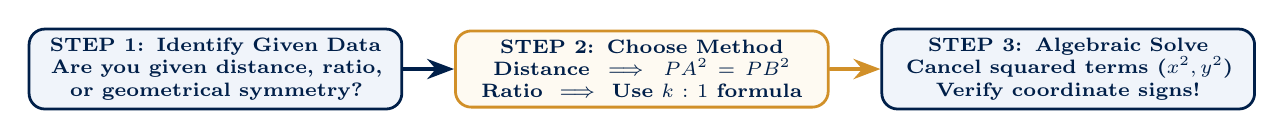
\begin{tikzpicture}[scale=0.95, line cap=round, line join=round]
  % Step 1
  \node[draw=primary, fill=primarylight, rounded corners=2mm, line width=1pt, font=\scriptsize\bfseries\color{navy}, align=center, text width=4.5cm] (Q1) at (0,2.5) {STEP 1: Identify Given Data\\Are you given distance, ratio,\\or geometrical symmetry?};

  % Step 2
  \node[draw=accent, fill=accentlight, rounded corners=2mm, line width=1pt, font=\scriptsize\bfseries\color{navy}, align=center, text width=4.5cm] (Q2) at (5.7,2.5) {STEP 2: Choose Method\\Distance $\implies PA^2 = PB^2$\\Ratio $\implies$ Use $k : 1$ formula};

  % Step 3
  \node[draw=primary, fill=primarylight, rounded corners=2mm, line width=1pt, font=\scriptsize\bfseries\color{navy}, align=center, text width=4.5cm] (Q3) at (11.4,2.5) {STEP 3: Algebraic Solve\\Cancel squared terms ($x^2, y^2$)\\Verify coordinate signs!};

  \draw[-{Stealth[scale=1.1]}, primary, line width=1.3pt] (Q1) -- (Q2);
  \draw[-{Stealth[scale=1.1]}, accent, line width=1.3pt] (Q2) -- (Q3);
\end{tikzpicture}
\end{center}

\vspace{0.8mm}
\begin{formulaBox}
  \textbf{Fast Mental Calculation Checks for Board Exams:}
  \begin{itemize}
    \item \textbf{Pythagorean Triplet Recognition:} Differences $|x_2 - x_1|$ and $|y_2 - y_1|$ matching $(3, 4) \implies d = 5$; $(5, 12) \implies d = 13$; $(7, 24) \implies d = 25$; $(8, 15) \implies d = 17$.
    \item \textbf{Circle Diameter Center:} The center of a circle is always the \textbf{midpoint of its diameter}: $C = \left(\frac{x_1+x_2}{2}, \frac{y_1+y_2}{2}\right)$. If center and one endpoint are given: $x_2 = 2x_C - x_1$, $y_2 = 2y_C - y_1$.
  \end{itemize}
\end{formulaBox}

\newpage

% =============================================================================
% PAGE 12: MODULE 11 — WORKED BOARD EXAM ARCHETYPES (FULL STEPS)
% =============================================================================
\thispagestyle{fancy}
\vspace*{0mm}

\chapterbanner{07}{COORDINATE GEOMETRY}{Module 11 $\vert$ Board Exam Archetypes: 3-Mark \& 4-Mark Stepwise Layout}{\ExamTag}

\subhead{Archetype A (3-Mark Board Model) $\vert$ Circle Diameter \& Missing Endpoint}

\begin{conceptBox}[title={Archetype A: Center of Circle as Diameter Midpoint},fonttitle=\bfseries\color{navy}]
  \textbf{Problem:} Find the coordinates of a point $A$, where $AB$ is the diameter of a circle whose centre is $(2, -3)$ and $B$ is $(1, 4)$.
  \par\vspace{0.6mm}\noindent
  \textbf{Step 1: State the geometric property [1 Mark]:}\\
  The centre of a circle $C$ is the midpoint of its diameter $AB$. Let the coordinates of point $A$ be $(x, y)$. The given endpoint is $B(1, 4)$, and the centre is $C(2, -3)$.
  \par\noindent
  \textbf{Step 2: Apply the midpoint formula [1 Mark]:}
  $$C(x_C, y_C) = \left( \frac{x + 1}{2}, \; \frac{y + 4}{2} \right) = (2, -3)$$
  \textbf{Step 3: Solve for $x$ and $y$ independently [1 Mark]:}
  $$\frac{x + 1}{2} = 2 \implies x + 1 = 4 \implies \mathbf{x = 3}$$
  $$\frac{y + 4}{2} = -3 \implies y + 4 = -6 \implies \mathbf{y = -10}$$
  \textbf{Final Statement:} The coordinates of point $A$ are $\mathbf{(3, -10)}$.
\end{conceptBox}

\vspace{1mm}
\subhead{Archetype B (4-Mark Board Model) $\vert$ Section Formula with $AP = \frac{3}{7}AB$}

\begin{conceptBox}[title={Archetype B: Ratio Decoding and Coordinate Determination},fonttitle=\bfseries\color{navy}]
  \textbf{Problem:} If $A(-2, -2)$ and $B(2, -4)$ are two points, find the coordinates of $P$ such that $AP = \frac{3}{7}AB$ and $P$ lies on the line segment $AB$.
  \par\vspace{0.6mm}\noindent
  \textbf{Step 1: Decode the internal division ratio $m_1 : m_2$ [1.5 Marks]:}\\
  We are given that $AP = \frac{3}{7}AB$. Since $P$ lies on the segment $AB$:
  $$PB = AB - AP = AB - \frac{3}{7}AB = \frac{4}{7}AB$$
  Now compute the ratio of the parts:
  $$\frac{AP}{PB} = \frac{\frac{3}{7}AB}{\frac{4}{7}AB} = \frac{3}{4} \implies \mathbf{m_1 : m_2 = 3 : 4}$$
  \textbf{\TrapTag\ Common Error Alert:} Many students mistakenly use $3 : 7$. The ratio is strictly $3 : 4$!
  \par\noindent
  \textbf{Step 2: Apply the section formula [1.5 Marks]:}
  Here $(x_1, y_1) = (-2, -2)$, $(x_2, y_2) = (2, -4)$, $m_1 = 3$, $m_2 = 4$.
  $$x = \frac{m_1 x_2 + m_2 x_1}{m_1 + m_2} = \frac{3(2) + 4(-2)}{3 + 4} = \frac{6 - 8}{7} = \mathbf{-\frac{2}{7}}$$
  $$y = \frac{m_1 y_2 + m_2 y_1}{m_1 + m_2} = \frac{3(-4) + 4(-2)}{3 + 4} = \frac{-12 - 8}{7} = \mathbf{-\frac{20}{7}}$$
  \textbf{Step 3: Concluding result [1 Mark]:}\\
  The coordinates of point $P$ are $\mathbf{\left(-\frac{2}{7}, -\frac{20}{7}\right)}$.
\end{conceptBox}

\newpage

% =============================================================================
% PAGE 13: MODULE 12 — CASE-STUDY & APPLIED CONTEXTUAL MODELING
% =============================================================================
\thispagestyle{fancy}
\vspace*{0mm}

\chapterbanner{07}{COORDINATE GEOMETRY}{Module 12 $\vert$ Applied Case-Study: Sports Ground Grid \& GPS Navigation}{\ExamTag}

\subhead{Case Study 1 $\vert$ Sports Day Relay Race on a Coordinate Grid}

To conduct sports day activities in a rectangular school ground $ABCD$, lines have been drawn with chalk powder at a distance of $1\text{ m}$ each. $100$ flower pots have been placed at a distance of $1\text{ m}$ from each other along $AD$, so that $AD = 100\text{ m}$.
\begin{itemize}
  \item Niharika runs $\frac{1}{4}\text{th}$ of the distance $AD$ on the $2\text{nd}$ line and posts a green flag.
  \item Preet runs $\frac{1}{5}\text{th}$ of the distance $AD$ on the $8\text{th}$ line and posts a red flag.
\end{itemize}

\begin{minipage}[c]{0.42\textwidth}
\centering
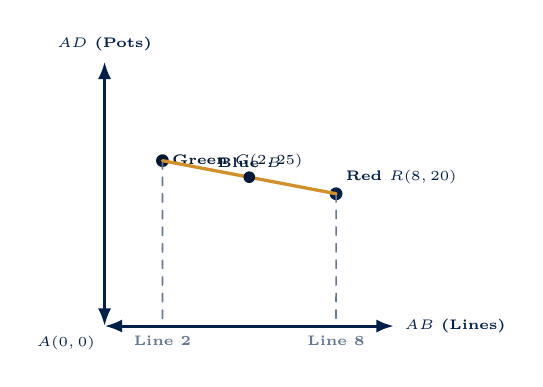
\begin{tikzpicture}[scale=1.05, line cap=round, line join=round]
  % Ground Axes
  \draw[{Latex[scale=0.8]}-{Latex[scale=0.8]}, primary, line width=1.1pt] (0,0) -- (3.5,0) node[right, font=\tiny\bfseries]{$AB$ (Lines)};
  \draw[{Latex[scale=0.8]}-{Latex[scale=0.8]}, primary, line width=1.1pt] (0,0) -- (0,3.2) node[above, font=\tiny\bfseries]{$AD$ (Pots)};
  \node[font=\tiny\bfseries\color{navy}, below left] at (0,0) {$A(0,0)$};

  % Green Flag G(2, 25)
  \coordinate (G) at (0.7,2.0);
  \fill[green!70!black] (G) circle (2.2pt) node[right, font=\tiny\bfseries\color{green!70!black}]{Green $G(2, 25)$};
  \draw[dashed, green!60, line width=0.6pt] (G) -- (0.7,0) node[below, font=\tiny\bfseries]{Line 2};

  % Red Flag R(8, 20)
  \coordinate (R) at (2.8,1.6);
  \fill[reddeep] (R) circle (2.2pt) node[above right, font=\tiny\bfseries\color{reddeep}]{Red $R(8, 20)$};
  \draw[dashed, reddeep!60, line width=0.6pt] (R) -- (2.8,0) node[below, font=\tiny\bfseries]{Line 8};

  % Line joining G and R
  \draw[accent, line width=1.2pt] (G) -- (R);

  % Blue Flag B at midpoint
  \coordinate (M) at (1.75,1.8);
  \fill[blue] (M) circle (2pt) node[above, font=\tiny\bfseries\color{blue}]{Blue $B$};
\end{tikzpicture}
\end{minipage}\hfill
\begin{minipage}[c]{0.56\textwidth}
\begin{conceptBox}[title={4-Mark Board Question Protocol},fonttitle=\bfseries\color{navy}]
  \textbf{Questions:}
  \begin{enumerate}
    \item Write the coordinates of the green flag $G$ and the red flag $R$. [1M]
    \item Find the straight-line distance between both flags. [1M]
    \item If Rashmi has to post a blue flag exactly halfway between the line segment joining the two flags, on which line and at what distance should she post her flag? [2M]
  \end{enumerate}
\end{conceptBox}
\end{minipage}

\vspace{0.8mm}
\begin{successBox}[title={Solution \& Marking Scheme Evaluation},fonttitle=\bfseries\color{navy}]
  \begin{enumerate}
    \item \textbf{Coordinates of Flags [1M]:}
      \begin{itemize}
        \item Green flag $G$: $x = 2$, $y = \frac{1}{4} \times 100 = 25 \implies \mathbf{G(2, 25)}$.
        \item Red flag $R$: $x = 8$, $y = \frac{1}{5} \times 100 = 20 \implies \mathbf{R(8, 20)}$.
      \end{itemize}
    \item \textbf{Distance Between Flags [1M]:}
      $$d = \sqrt{(8 - 2)^2 + (20 - 25)^2} = \sqrt{6^2 + (-5)^2} = \sqrt{36 + 25} = \mathbf{\sqrt{61}\text{ m}} \approx 7.81\text{ m}$$
    \item \textbf{Position of the Blue Flag [2M]:}
      The blue flag is posted at the \textbf{midpoint} of $GR$:
      $$M = \left( \frac{2 + 8}{2}, \; \frac{25 + 20}{2} \right) = \left( \frac{10}{2}, \; \frac{45}{2} \right) = \mathbf{(5, 22.5)}$$
      \textbf{Answer:} Rashmi should post her blue flag on the \textbf{$5\text{th}$ line} at a distance of \textbf{$22.5\text{ m}$}.
  \end{enumerate}
\end{successBox}

\newpage

% =============================================================================
% PAGE 14: MODULE 13 — BOARD EXAM TRAPS, HACKS & PRE-SUBMISSION AUDIT
% =============================================================================
\thispagestyle{fancy}
\vspace*{0mm}

\chapterbanner{07}{COORDINATE GEOMETRY}{Module 13 $\vert$ Board Traps, Verification Hacks \& 5-Point Audit}{\ExamTag}

\subhead{13.1 The Top 7 Coordinate Geometry Board Traps (And How to Bust Them)}

\begin{enumerate}[label=\textbf{Trap \arabic*:}, leftmargin=5mm, itemsep=1pt, topsep=0.8pt, parsep=0pt]
  \item \textbf{The Negative Sign Subtraction Trap:} In $(x_2 - x_1)$, when $x_1$ is negative, writing $x_2 - x_1$ as $x_2 - 5$ instead of $x_2 - (-5) = \mathbf{x_2 + 5}$. \TrapTag\ Always enclose negative coordinates in parentheses!
  \item \textbf{The Section Formula Cross-Index Confusion:} Multiplying $m_1$ with $x_1$ instead of $x_2$. Remember the criss-cross rule: $\mathbf{m_1}$ multiplies with the \textbf{opposite point $(x_2, y_2)$}.
  \item \textbf{Axis Coordinate Mix-up:} Assuming a point on the $y$-axis is $(y, 0)$. A point on the \textbf{$y$-axis has $x = 0$}, so it is strictly $\mathbf{(0, y)}$. A point on the $x$-axis is $\mathbf{(x, 0)}$.
  \item \textbf{The Trisection $1:3$ Error:} Believing trisection means ratio $1 : 3$. Three equal parts means the internal ratios are strictly $\mathbf{1 : 2}$ and $\mathbf{2 : 1}$!
  \item \textbf{Squaring Incomplete Binomials:} Expanding $(x - 3)^2$ as $x^2 - 9$ or $x^2 + 9$ instead of $\mathbf{x^2 - 6x + 9}$.
  \item \textbf{Parallelogram Cyclic Order Violation:} Taking vertices out of order (e.g., across diagonals). Vertices $A, B, C, D$ must be taken in \textbf{continuous cyclic order} along the perimeter.
  \item \textbf{The Deleted Triangle Area Formula Trap:} Using the triangle area formula $\frac{1}{2}|x(y-y) + \dots|$ to prove collinearity. This formula is \textbf{deleted from the CBSE syllabus}; use the \textbf{Distance Sum Rule} ($AB + BC = AC$).
\end{enumerate}

\subhead{13.2 High-Speed Algebraic Verification Protocol}

\begin{tabularx}{\textwidth}{X | X}
\toprule
\rowcolor{redpale}
\textbf{The Slow Method (High Risk of Arithmetic Slip)} & \textbf{The Maths Manthan Factoring Method} \\
\midrule
Finding 4th vertex of parallelogram $ABCD$: & Use the common diagonal midpoint property: \\
Set up distance equations: $AB = CD$ and $BC = DA$. & $\text{Midpoint}(AC) = \text{Midpoint}(BD)$ \\
Leads to complicated non-linear simultaneous radical equations requiring quadratic substitution. & $x_1 + x_3 = x_2 + x_4 \implies \mathbf{x_4 = x_1 + x_3 - x_2}$ \\
Time taken: $\approx 5\text{ minutes}$. & $y_1 + y_3 = y_2 + y_4 \implies \mathbf{y_4 = y_1 + y_3 - y_2}$ \\
Arithmetic error rate: $> 35\%$. & \textbf{Solves in 10 seconds with 100\% certainty!} \\
\bottomrule
\end{tabularx}

\vspace{1mm}
\subhead{13.3 The 5-Point Board Examination Pre-Submission Checklist}

\begin{successBox}[top=1.2mm,bottom=1.2mm,before skip=1.5pt,after skip=1pt]
  \textbf{Final 60-Second Answer Sheet Verification Protocol:}
  \begin{itemize}[leftmargin=4mm,itemsep=1pt,topsep=1pt,parsep=0pt]
    \item[$\square$] \textbf{Coordinates Stated with Signs:} Did you double check that $(x_2 - x_1)$ correctly handled negative signs with double parentheses?
    \item[$\square$] \textbf{Symbolic Formula Stated:} Did you write $d = \sqrt{(x_2-x_1)^2+(y_2-y_1)^2}$ or the section formula before substituting values? (Guarantees CBSE method marks).
    \item[$\square$] \textbf{Squared Distances Equated:} For equidistant questions ($PA = PB$), did you write $PA^2 = PB^2$ to cleanly justify eliminating square roots?
    \item[$\square$] \textbf{Ratio Stated Correctly:} Did you confirm whether the question asked for $m_1 : m_2$ (parts of segment) or coordinates of the point?
    \item[$\square$] \textbf{Geometric Units Attached:} Are final linear distances labeled with $\mathbf{\text{units}}$?
  \end{itemize}
\end{successBox}

\vfill
\begin{center}
  {\footnotesize\bfseries\color{primary}MATHS MANTHAN TUITION CLASSES \quad$\vert$\quad END OF CHAPTER 7 HANDBOOK}\\[1mm]
  {\scriptsize\color{secondary}Designed for Academic Excellence in CBSE Class 10 Board Examinations 2026--27.}
\end{center}

\end{document}
